
\section{\ref{PS:Q:Availability}}
\subsection{Experiment}
The \ref{PS:Q:Availability} question asks if the proposed decentralized system is able to continue its functions even though nodes are removed from the system at runtime.
The proposed decentralized system should be able to continue maintaining the global setpoint of the park even if some turbines become unavailable, this of course assumes that available capacity is present in the park.

The below experiment is repeated with a N failing turbines
The experiment has the following procedure:
$N = 1, 5, 10, 15$
\begin{enumerate}
	\item Start the system with 30 turbines.
	\item Make sure the system is stable.
	\item Kill N nodes.
	\begin{itemize}
		\item did the system discover the failed node within a 150ms timeframe?
		\item did the system adjust the setpoints for all turbines to maintain the global setpoint?
	\end{itemize}
\end{enumerate}

\subsection{Results}
\label{sec:res:availability}
The plots in \cref{fig:exp:availability_kill15,fig:exp:availability_kill10,fig:exp:availability_kill5,fig:exp:availability_kill1} show how the decentralized solution reacts when killing 1, 5, 10 and 15 turbines. To begin with there are 30 turbines, the setpoint is set to 2,000 for all setups except for when killing only one turbine(\cref{fig:exp:availability_kill1}) it was set to 20,000. This was done so that it was possible to visually verify that the turbines reacted.
The turbines are all running with a cycle time of 20 ms.

\begin{figure}
	\centering
	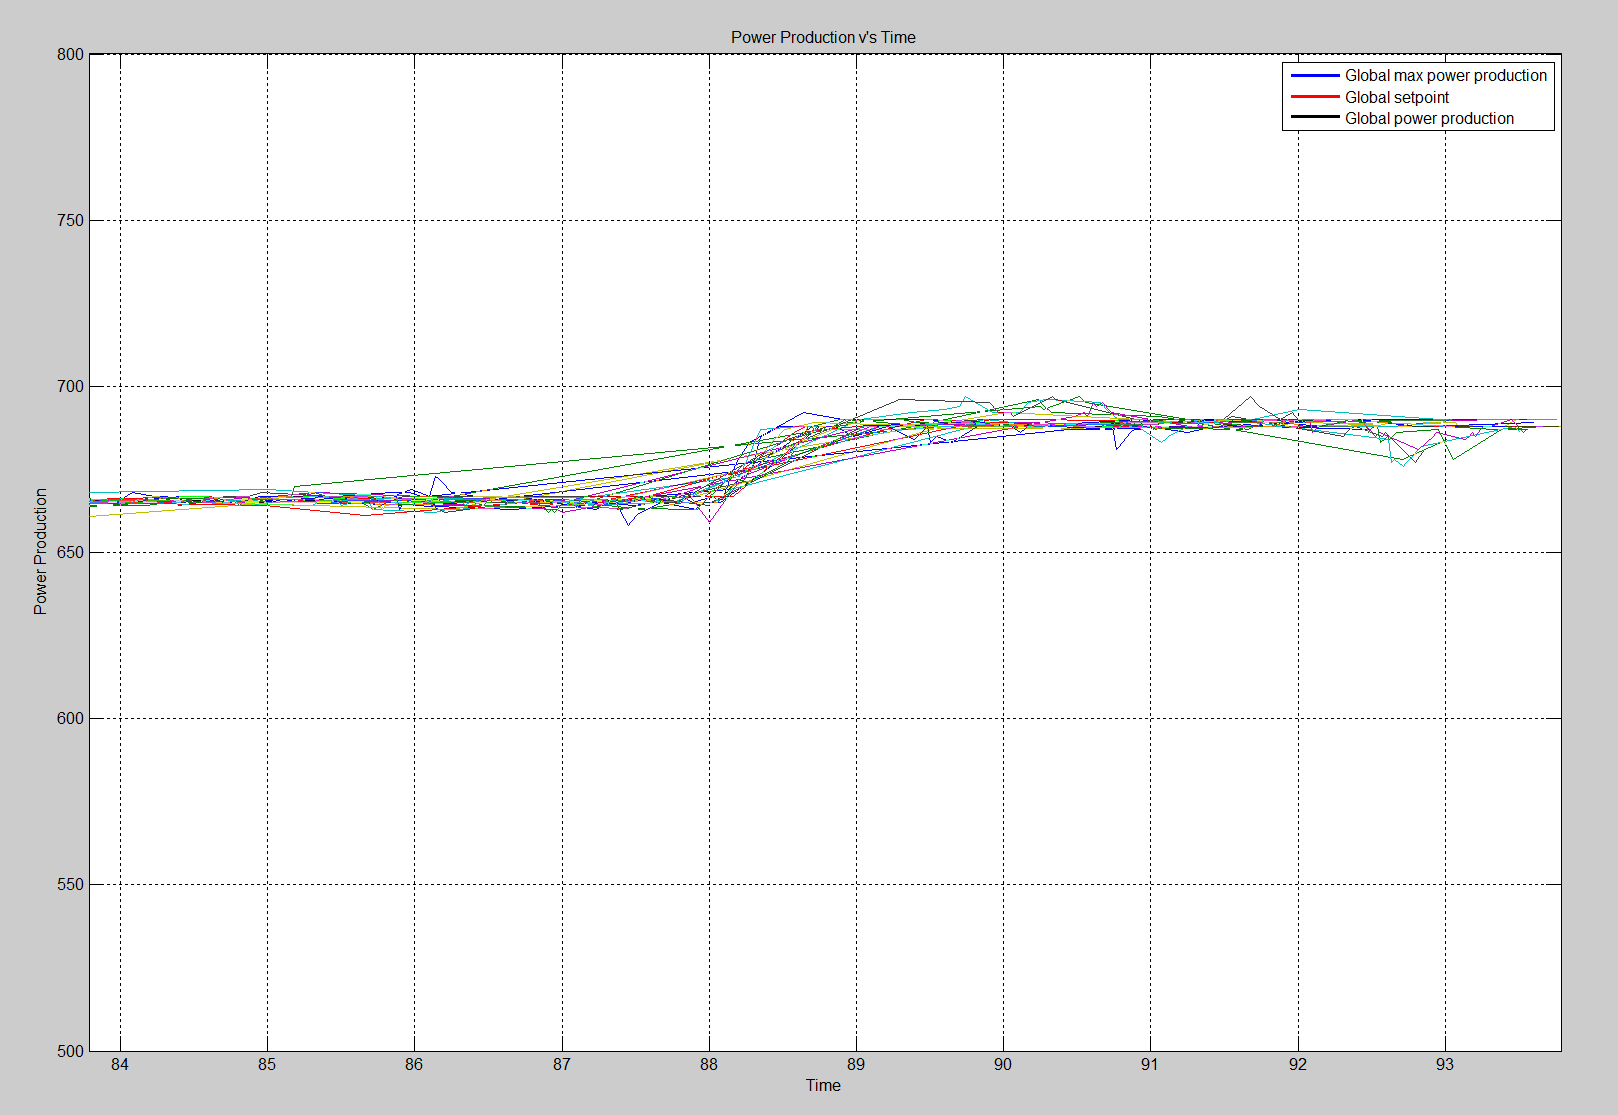
\includegraphics[width=\resultsFigureWidthScale\textwidth]{figures/Results/availabilitytest30-29_setpoint_20000.PNG}
	\caption{Availability test kill 1 out of 30 turbines}
	\label{fig:exp:availability_kill1}
\end{figure}

\begin{figure}
	\centering
	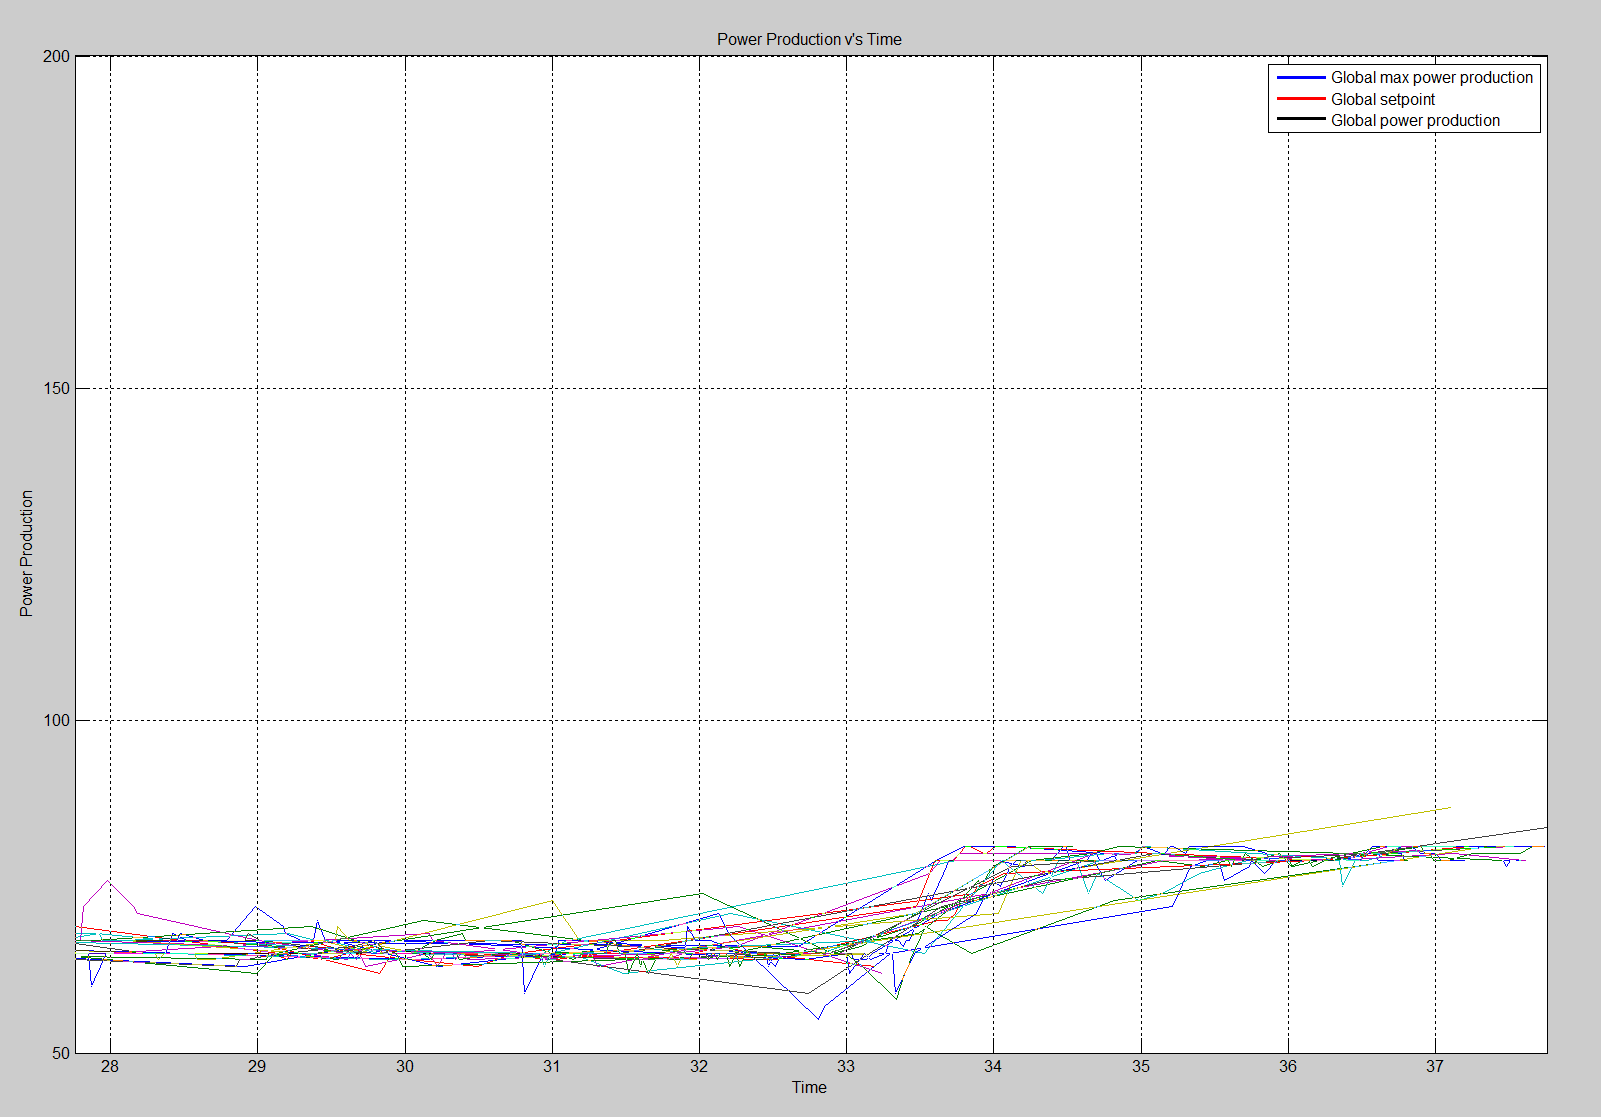
\includegraphics[width=\resultsFigureWidthScale\textwidth]{figures/Results/availabilitytest30-25_setpoint_2000.PNG}
	\caption{Availability test kill 5 out of 30 turbines}
	\label{fig:exp:availability_kill5}
\end{figure}

\begin{figure}
	\centering
	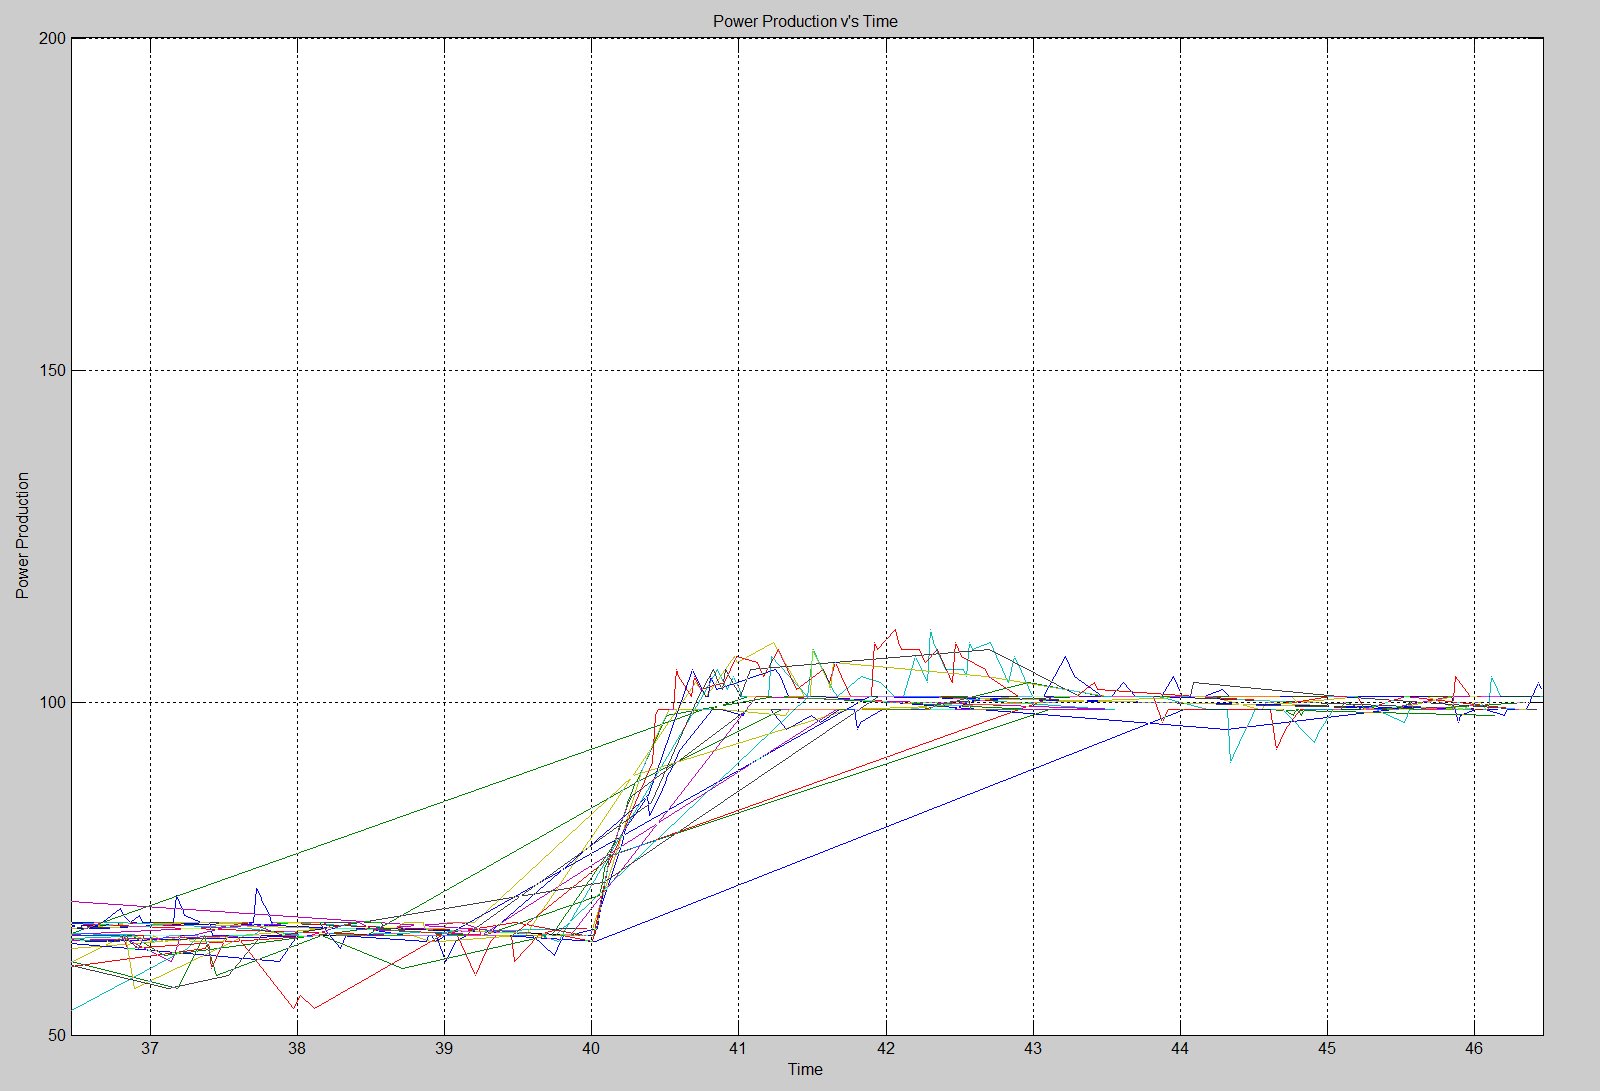
\includegraphics[width=\resultsFigureWidthScale\textwidth]{figures/Results/availabilitytest30-20_setpoint_2000.PNG}
	\caption{Availability test kill 10 out of 30 turbines}
	\label{fig:exp:availability_kill10}
\end{figure}

\begin{figure}
	\centering
	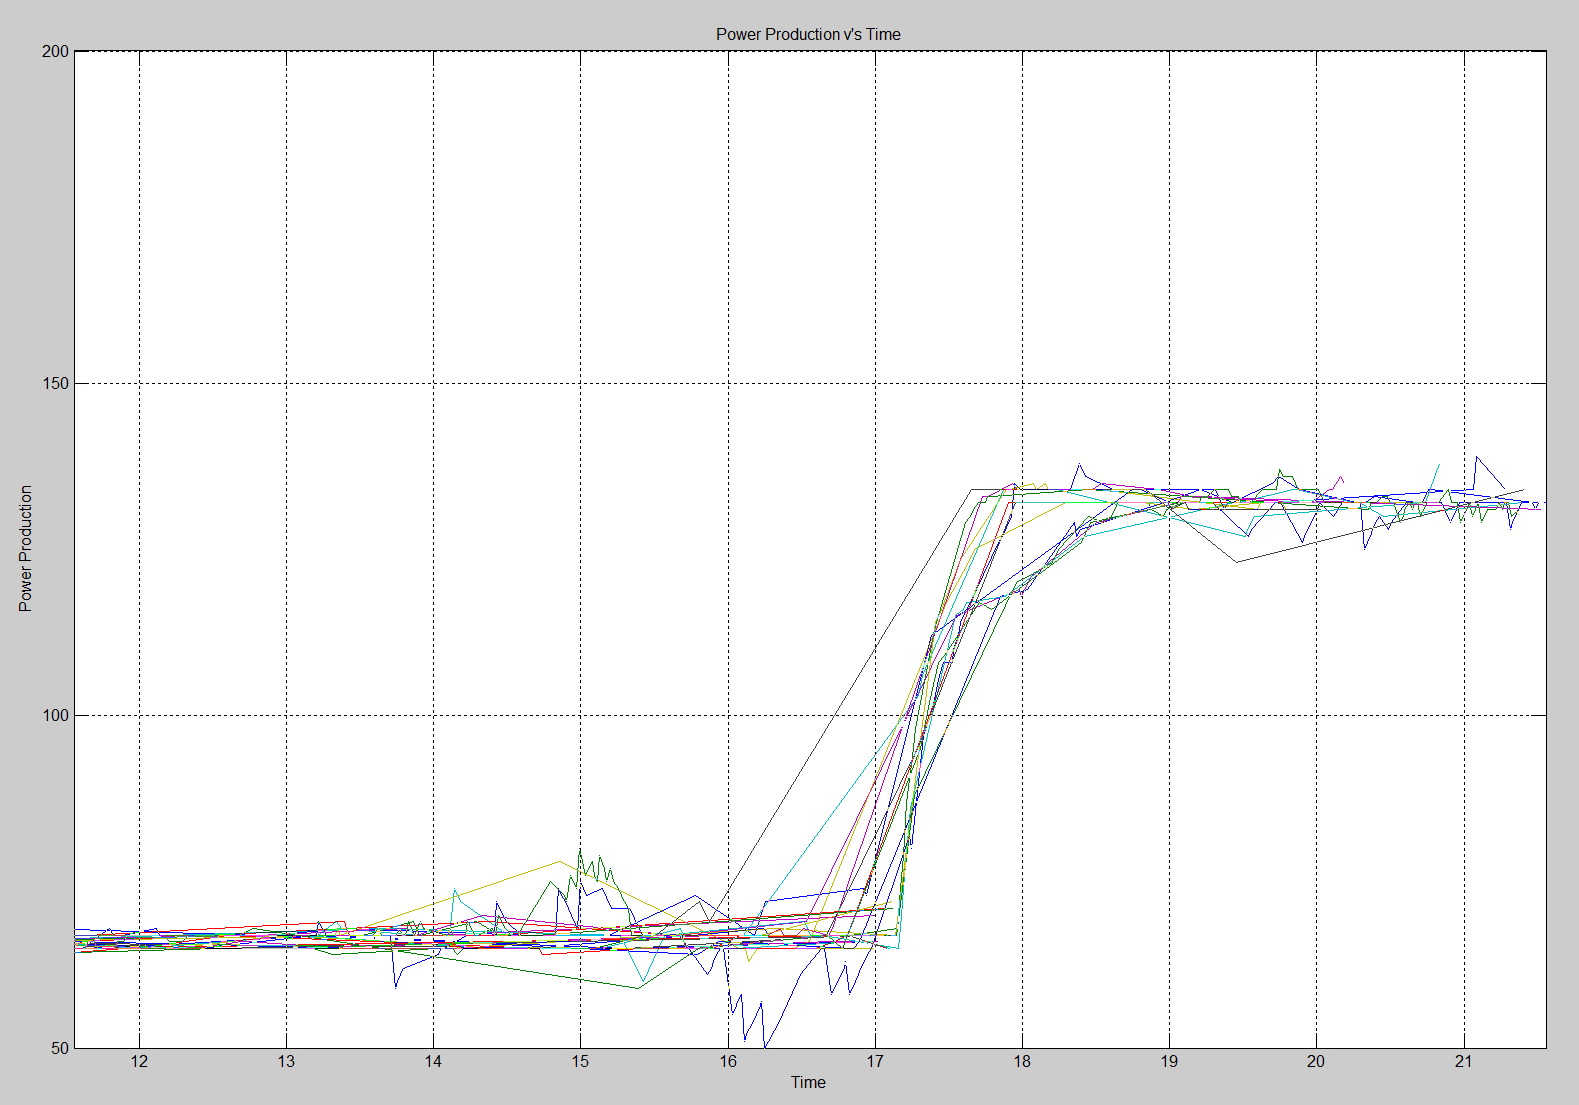
\includegraphics[width=\resultsFigureWidthScale\textwidth]{figures/Results/availabilitytest30-15_setpoint_2000.PNG}
	\caption{Availability test kill 15 out of 30 turbines}
	\label{fig:exp:availability_kill15}
\end{figure}


\subsection{Discussion}
One of the main challenges of decentralized systems is to continue operation in the face of communication failure or node loss. This section address the \ref{PS:Q:Availability} problem of \cref{sec:problemStatement} which deal with the availability of the decentralized solution.

As presented in figures \ref{fig:exp:availability_kill1} to \ref{fig:exp:availability_kill15} the decentralized solution can handle the loss of turbines. A turbine is considered offline if it does not publish any new data to any other turbines within a 150 ms timespan as defined by the History QoS parameter described in \cref{sec:decen:ddsconf}.
This upper limit of 150 ms is chosen because this is the upper limit of the regulation cycle time in the current Simens system.
After the turbine has been detected as offline the remaining turbines in the wind farm will share the load of the missing turbines to keep the global power production of the park as close to the global setpoint as possible. The removal of one turbine from the windfarm is illustrated in \cref{fig:exp:availability_kill1}.

Removing several turbines from the system does not impede the regulation of the wind farm either. The remaining turbines will share the extra load between themselves and continue power production. The removal of several turbines are illustrated in figures \ref{fig:exp:availability_kill5} to \ref{fig:exp:availability_kill15}.

%The time it takes the decentralized solution to detect a turbine loss and recover power production is dependent on the following parameters:
%
%\begin{itemize}
%	\item Time of turbine loss detection, which is defined by the History QoS to 150 ms, $I$.
%	\item Time between regulation cycles, in the test cases presented in \cref{sec:res:availability} the time is set to 20 ms, $S$.
%	\item Time of calulation of a new setpoint, $C$.
%	\item Time for the turbine to regulate power production according to the new setpoint. In the turbines this process is simulated with a simple regulation that may take several regulation cycles to complete $R$.
%\end{itemize}
%
%Thus the time for recovery of the power production when a turbine failure occurs can be calculated as $T = I + S + C + R$ which translates to $150 ms + 20 ms + C + R = 170 + C + R ms$. This time can be reduced by lowering the time it takes to detect a turbine is offline which increases the likelihood of detecting a delayed turbine as offline, or by lowering the time between regulation cycles which increases the likelihood of cache reads.

Internal communication and regulation are only two parameters of availability though. To ensure that the wind farm is reachable from the outside world in the face of turbine failure, sets special requirements to the component chosen to handle external communication. A component capable of handling this specific problem has been described in \cref{cha:resourceManagement}.

We also need to address the problem of data loss when a turbine is unresponsive. A turbine has several control and measurement points which are continually logged to a local data store. Should a turbine break down the local data may be destroyed with the turbine. This again sets special requirements to the component handling data storage. In \cref{sec:databaseStorage} the requirements to the data storage component is described and MongoDB was presented as the best choice to solve the availability problem of data storage. MongoDB is capable of automatic replication of data between turbines such that data is still available should a turbine failure occur. As well as replication MongoDB provides automatic sharding of a database which enables global data to be stored across a number of nodes such that no single node contains all global data. Furthermore MongoDB supports aggregation of data across turbines to calculate aggregated values as for instance the global production of the wind farm.

Making the decentralized solution robust and able to handle the loss of turbines with regards to internal communication, regulation of power production, external communication and data storage increases the overall availability of the wind farm. 
